\section{Random-submission floor}
\label{app:floor}

This appendix calibrates the directed-F1 axis used in Section~\ref{sec:results}. Because directed F1 (Appendix~\ref{app:scoring:directed}) is bounded below by what a structure-blind submitter achieves rather than by zero, an absolute score has no fixed meaning across levels: the ladder varies graph density and the floor varies with it. C.1--C.2 give the sampler and its closed-form expected F1; C.3 confirms the closed form against direct simulation; C.4 plots the curve with the v1 ladder range shaded; C.5 lists the per-level floors a reader needs to subtract from a §\ref{sec:results} number before drawing a conclusion.

\subsection{Random-submission policy}
\label{app:floor:policy}

The policy is the \emph{uniform-$m$ random DAG} sampler of \texttt{make\_random\_uniform\_submission} (\texttt{run\_random\_dag\_baseline.py:200--217}). It uses only the public node count $d$; it does not call \texttt{observe()} or \texttt{intervene()}, does not consult the CPDAG or the true edge count $k$, and submits no undirected edges. With $M = d(d-1)/2$:
\begin{enumerate}
\itemsep0pt
\item Draw a topological order $\pi \sim \mathrm{Uniform}(S_d)$.
\item Draw $m \sim \mathrm{Uniform}\{0, 1, \ldots, M\}$.
\item Sample $m$ edges uniformly without replacement from the $M$ order-respecting candidate pairs $\{(\pi(i), \pi(j)) : i < j\}$ and submit them as $E_d$, with $E_u = \emptyset$.
\end{enumerate}
The resulting submission is a DAG by construction (it respects $\pi$); it is scored by the same \texttt{score\_submission} as any LLM or PC submission.

\subsection{Closed-form expected directed F1}
\label{app:floor:closed}

Let $G$ be the true DAG with $|E(G)| = k$ edges. Consider one true directed edge $(u, v) \in E(G)$. Under the sampler of C.1, the unordered pair $\{u, v\}$ appears among the $m$ chosen pairs with probability $m/M$ by symmetry of uniform sampling without replacement. Conditional on inclusion, the orientation in the submission is $(u, v)$ iff $\pi$ places $u$ before $v$, which happens with probability $1/2$ under uniform $\pi$. Therefore
\begin{equation}
\Pr\bigl[(u, v) \in E_d(\mathcal{S}) \,\big|\, m\bigr] = \frac{m}{2M},
\qquad
\mathbb{E}[\,|E_d(\mathcal{S}) \cap E(G)| \,\big|\, m\,] = \frac{km}{2M}.
\end{equation}
With $|E_d(\mathcal{S})| = m$ and $|E(G)| = k$ deterministic given $(m, k)$, the per-$m$ directed precision and recall are $\mathbb{E}[\mathrm{TP}|m]/m = k/(2M)$ and $\mathbb{E}[\mathrm{TP}|m]/k = m/(2M)$, giving the harmonic mean
\begin{equation}
\mathbb{E}[F_1 \mid m, k] \;=\; \frac{km}{M(m + k)}.
\end{equation}
Averaging uniformly over $m$ yields the discrete closed form
\begin{equation}
\mathbb{E}[F_1 \mid d, k] \;=\; \frac{1}{M+1} \sum_{m=0}^{M} \frac{k\,m}{M\,(m + k)},
\label{eq:floor-closed}
\end{equation}
implemented verbatim in \texttt{exact\_expected\_directed\_f1} (\texttt{scripts/ladder\_random\_floor\_sanity.py:65--72}).

\subsection{Empirical confirmation}
\label{app:floor:empirical}

The probe draws $16 \times 100 = 1600$ uniform-$m$ submissions per level, scores each through the canonical \texttt{score\_submission}, and reports the per-level mean and standard error. The \texttt{v0\_like\_density\_probe} rows of \texttt{traces/ladder\_random\_floor\_sanity/summary.csv} cover L1--L4 at the production $(d, k)$; the L5 entry is measured separately at the production $(d, k) = (14, 16)$ with the same protocol.

\begin{center}
\small
\begin{tabular}{@{}l c c c c c@{}}
\toprule
Level & $(d, k)$ & $\rho$ & $\mathbb{E}[F_1]$ (closed) & Measured $\pm$ SE & Gap \\
\midrule
L1 & $(6, 6)$   & $0.400$ & $0.1957$ & $0.1923 \pm 0.0041$ & $-0.0034$ \\
L2 & $(8, 9)$   & $0.321$ & $0.1734$ & $0.1765 \pm 0.0031$ & $+0.0030$ \\
L3 & $(10, 12)$ & $0.267$ & $0.1547$ & $0.1527 \pm 0.0025$ & $-0.0020$ \\
L4 & $(12, 14)$ & $0.212$ & $0.1330$ & $0.1350 \pm 0.0020$ & $+0.0021$ \\
L5 & $(14, 16)$ & $0.176$ & $0.1166$ & $0.1144 \pm 0.0017$ & $-0.0022$ \\
\bottomrule
\end{tabular}
\end{center}

The gap is within $1.3$ standard errors on every row, confirming Equation~\eqref{eq:floor-closed}.

\subsection{Floor curve}
\label{app:floor:figure}

\begin{figure}[h]
\centering
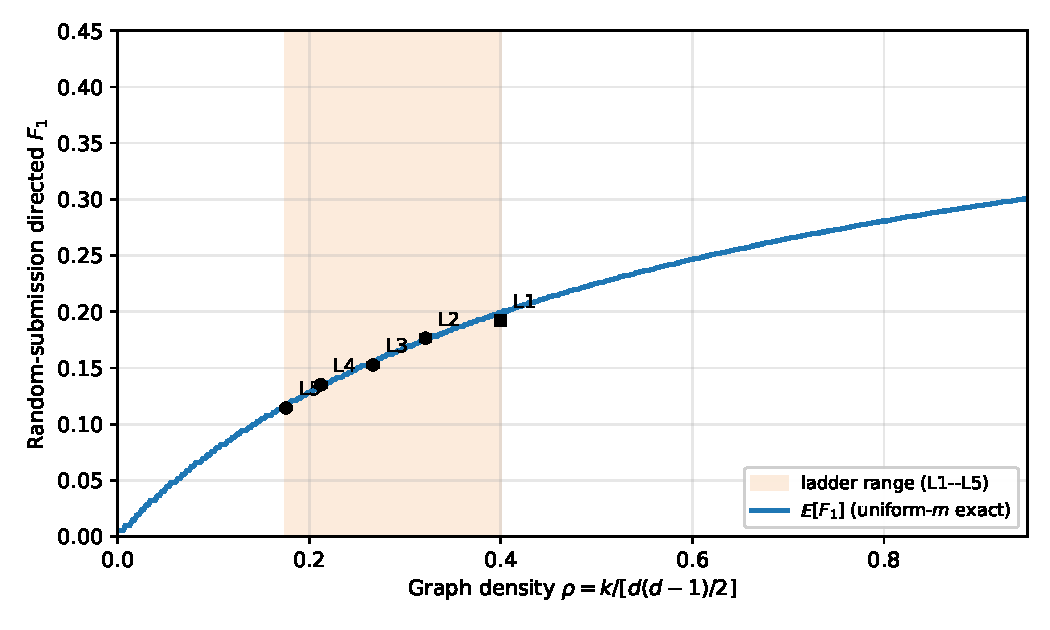
\includegraphics[width=0.95\linewidth]{figures/generated/fig_random_floor.pdf}
\caption{Random-submission directed-F1 floor as a function of graph density $\rho$. Solid: closed-form $\mathbb{E}[F_1]$ (Equation~\eqref{eq:floor-closed}, evaluated at a reference $d = 20$; the curve is essentially flat in $d$ once $d \ge 12$). Black dots with error bars: measured per-level means $\pm$ SE for L1--L5 from the probe of C.3. The shaded band marks the ladder density range; results in Section~\ref{sec:results} should be read as gap above this floor at the level's density, not as absolute $F_1$.}
\label{fig:random-floor}
\end{figure}

\subsection{Reading Section~\ref{sec:results} against the floor}
\label{app:floor:reading}

The per-level closed-form floors at the production $(d, k)$ of \texttt{ladder\_levels\_v1} (\texttt{run\_ladder.py:124--132}) are
\begin{equation*}
\text{L1: } 0.196, \quad
\text{L2: } 0.173, \quad
\text{L3: } 0.155, \quad
\text{L4: } 0.133, \quad
\text{L5: } 0.117.
\end{equation*}
A model F1 of $0.30$ is a $+0.10$ gap at L1 and a $+0.18$ gap at L5; the cross-level comparison that matters is the gap, not the absolute. We therefore report gap-above-floor alongside raw F1 in the per-model tables of Appendix~\ref{app:results}.
